% % % % % % % % % % % % % % % % % % % % % % % % % % % % % % % % % % % % % % % % % % % %
%                                                                                     %
% Short Sectioned Assignment LaTeX Template Version 1.0 (5/5/12)                      %
% This template has been downloaded from: http://www.LaTeXTemplates.com               %
%                                                                                     %
% Original author:  Frits Wenneker (http://www.howtotex.com)                          %
%                                                                                     %
% Modified by: Fco Javier Sueza Rodríguez (fcosueza@disroot.org)                      %
%                                                                                     %
% Changes:                                                                            %
%	    - Custom Chapters, Sections and Subsections (titlesec package)                %
%           - Document type scrbook (oneside)                                         %
%           - Use babel-lang-spanish package and marvosym                             %
%           - Use hyperref, enumitem, tcolorbox and glossaries packages               %
%           - Use Time New Roman (mathptmx), Helvetic and Courier fonts               %
%                                                                                     %
% License: CC BY-NC-SA 3.0 (http://creativecommons.org/licenses/by-nc-sa/3.0/)        %
%                                                                                     %
% % % % % % % % % % % % % % % % % % % % % % % % % % % % % % % % % % % % % % % % % % % %

%-----------------------------------------------%
%	              Packages                  %
%-----------------------------------------------%

\documentclass[paper=a4, fontsize=11pt, oneside]{scrbook}

% ---- Text Input/Output ----- %

\usepackage[T1]{fontenc}
\usepackage[utf8]{inputenc}
\usepackage{mathptmx}
\usepackage[scaled=.92]{helvet}
\usepackage{courier}
\usepackage[indent=12pt]{parskip}

\usepackage{geometry}
\geometry{verbose,tmargin=3cm,bmargin=3cm,lmargin=2.6cm,rmargin=2.6cm}

% ---- Language ----- %

\usepackage[spanish]{babel}
\usepackage{marvosym}

% ---- Another packages ---- %

\usepackage{amsmath,amsfonts,amsthm}
\usepackage{graphics,graphicx}
\usepackage{titlesec}
\usepackage{fancyhdr}
\usepackage{tcolorbox}
\usepackage{hyperref}
\usepackage{enumitem}
\usepackage[automake]{glossaries}

%--------------------------------------------------------------------%
%                      Customizing Document                          %
%--------------------------------------------------------------------%


% ----------- Custom Chapters, Sections and Subsections -------------- %

\titleformat{\chapter}[display]
			{\bfseries\Huge}
			{Tema \ \thechapter} {0.5ex}
			{\vspace{1ex}\centering}

\titleformat{\section}[hang]
			{\bfseries\Large}
			{\thesection}{0.5em}{}

\titleformat{\subsection}[hang]
			{\bfseries\large}
			{\thesubsection}{0.5em}{}

\titleformat{\subsubsection}[hang]
			{\bfseries\large}
			{\thesubsubsection}{0.5em}{}

\hypersetup{
    colorlinks=true,
    linkcolor=black,
    urlcolor=magenta
}

% ------------------- Custom heaaders and footers ------------------- %

\pagestyle{fancyplain}

\fancyhead[]{}
\fancyfoot[L]{}
\fancyfoot[C]{}
\fancyfoot[R]{\thepage}

\renewcommand{\headrulewidth}{0pt} % Remove header underlines
\renewcommand{\footrulewidth}{0pt} % Remove footer underlines

\setlength{\headheight}{13.6pt} % Customize the height of the header

% --------- Numbering equations, figures and tables ----------------- %

\numberwithin{equation}{section} % Number equations within sections
\numberwithin{figure}{section} % Number figures within sections
\numberwithin{table}{section} % Number tables within sections

% ------------------------ New Commands ----------------------------- %

\newcommand{\horrule}[1]{\rule{\linewidth}{#1}} % Create horizontal rule command


%----------------------------------------------------------------------------------------
%	TÍTULO Y DATOS DEL ALUMNO
%----------------------------------------------------------------------------------------

\title{
\normalfont \normalsize
\textsc{{\bfseries Curso 2023-2024} \\ Ciclo Superior de Desarrollo de Aplicaciones Web \\ IES Aguadulce} \\ [25pt]
\horrule{0.5pt} \\[0.4cm]
\huge Desarrollo de Interfaces Web \\
\horrule{0.5pt} \\[0.4cm]
}

\author{Francisco Javier Sueza Rodríguez}
\date{\normalsize\today}

%----------------------------------------------------------------------------------------
%                                     DOCUMENTO
%----------------------------------------------------------------------------------------
\makeglossaries
\loadglsentries{glossary.tex}

\begin{document}

\maketitle

\newpage

\tableofcontents

\listoffigures

%\listoftables

\newpage

\chapter{Planificación de Interfaces Web}
En este primer tema, vamos a estudiar en que consiste una interfaz web, viendo cuales son sus elementos  y las principales características que deben tener. Además, veremos conceptos básicos de diseño, haciendo hincapié en los principio de Gestalt, el color, las fuentes y otros elementos imprescindibles de una interfaz. También veremos que son las Guías de Estilo como nos pueden ayudar en el proceso de implementación de una interfaz.

\section{Elementos de Diseño}
Las personas del mundo civilizado vividos rodeadas de objetos que han sido fruto del diseño. Desde la silla donde te sientas, el microondas donde calientas la comida o la cafetera donde te haces el café. Todas y cada una de las cosas que nos rodean han pasado un proceso de diseño para lograr lo que se pretendía con su fabricación: funcionalidad, comodidad, atractivo, etc...

Utilizado normalmente en el contexto de las artes, ingeniería, arquitectura y otras disciplinas, \textbf{diseño} se define como el proceso previo de configuración mental en la búsqueda de una solución en cualquier campo.

Diseñar requiere principalmente consideraciones estéticas y funcionales. Esto necesita numerosas fase de análisis, modelado, ajustes, y adaptaciones previas a la producción definitiva del objeto. Además comprende multitud de disciplinas y oficios dependiendo del objeto que se quiere crear.

Las personas dedicadas al diseño deben comunicar sus ideas y conceptos de una forma clara y directa por medio de los elementos gráficos. La eficacia de esta comunicación dependerá de los elementos que se emplee y en conocimiento que se tenga de ellos.

\subsection{Percepción Visual}

La \textbf{percepción} es el proceso de recogida y tratamiento de la información sensorial. Consiste en recibir, a través de los sentidos las imágenes, sonidos, impresiones y sensaciones externas y elaborar e interpretar esa información.

La \textbf{percepción visual} es la sensación interior de conocimiento aparente que resulta de un estímulo o impresión luminosa registrada por nuestros ojos.

Existe una teoría (\textbf{psicología de Gestalt}) de la percepción, que estudia como nuestro cerebro decodifica la información recibida, a través de diversas asociaciones que se producen en el momento de la percepción. Según esta teoría, la mente configura, a través de ciertas leyes, los elementos que le llegan a través de los canales sensoriales o a través de la memoria.

Toda percepción es una acto de búsqueda de significado, no es recibir pasivamente la información, sino que implica buscar, seleccionar, relacionar, organizar, establecer conexiones, recordad, evaluar, etc...

En este aspecto, los diseñadores son comunicadores visuales, por lo que deben conocer al público, sus necesidades e inquietudes, para poder lograr que el mensaje visual llegue de forma correcta al receptor.

\subsection{Elementos Conceptuales: Punto, Línea, Plano y Volumen}
Los \textbf{elementos conceptuales} del diseño son la base del mismo, donde se asientan los demás elementos que veremos a continuación. Cada uno tiene sus propias características que les permite desempeñar unas funciones determinadas dentro de una composición.

\begin{itemize}
    \item \textbf{Punto}: es el resultado del primer encuentro de la punta del lápiz con el papel, tela u otro material. El \textbf{punto} es concebido en la imaginación pequeño y redondo. Un punto indica posición. No tiene largo ni ancho y es el principio y el fin de una línea y la intersección de dos líneas.

    \begin{figure}[H]
        \centering
        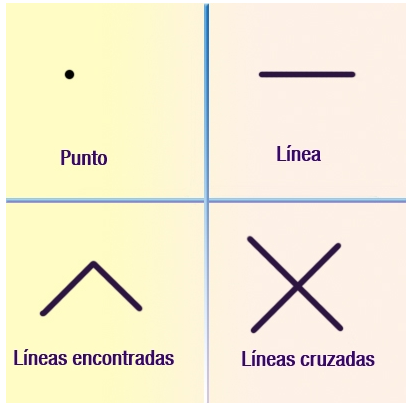
\includegraphics[scale=0.32]{el-punto.png}
    \end{figure}

    \item \textbf{Línea}: la línea no es visible por sí sola en la naturaleza. Es el resultado del movimiento de un punto que se desplaza por una superficie. La línea tiene largo pero no ancho y tiene dirección y posición. Esta limitad por dos puntos siendo esta la distancia más corta entre ambos. La línea delimita el espacio dando lugar a formas, representa el perfil o contorno de las cosas.

    \begin{figure}[H]
        \centering
        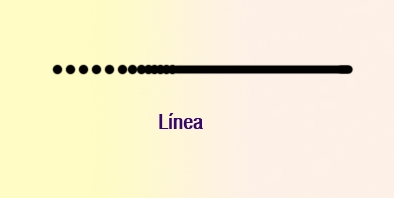
\includegraphics[scale=0.35]{la-linea.png}
    \end{figure}

    \item \textbf{Plano}: es el resultado del movimiento de una línea en dirección contraria a la suya. Un plano tiene largo y ancho pero no alto. Es la porción de superficie limitada por una línea cerrada. Define los límites extremos de un volumen.

    \begin{figure}[H]
        \centering
        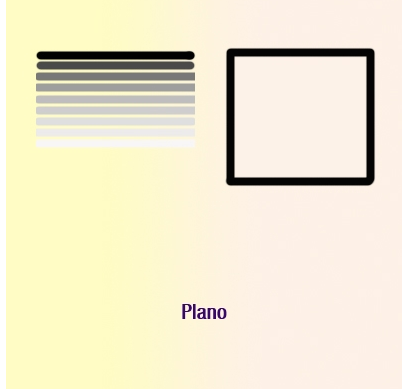
\includegraphics[scale=0.35]{el-plano.png}
    \end{figure}

    \item \textbf{Volumen}: es el resultado del movimiento de un plano que se desplaza en un dirección diferente a la suya. Tiene una posición en el espacio y esta limitado por planos. En un diseño bidimensional, el volumen es ilusorio.

    \begin{figure}[H]
        \centering
        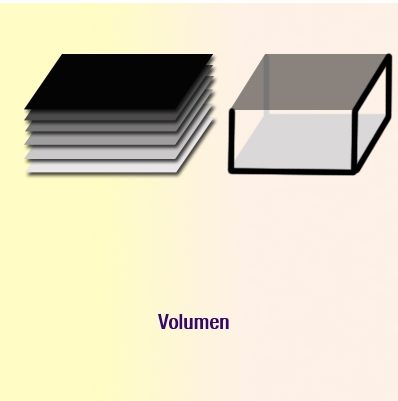
\includegraphics[scale=0.35]{el-volumen.png}
    \end{figure}
\end{itemize}

\subsection{Elementos Visuales: Forma, Medida, Color y Textura}
Los \textbf{elementos visuales} son la parte más importa de un diseño, porque son realmente lo que vemos.

Cuando dibujamos una línea en un papel empleamos una línea visible para representar la línea conceptual. Ésta tiene largo y ancho, y su color y textura vendrán determinados por el material empleado para representarla. Así, cuando lo elementos conceptuales se hacen visibles, estos tendrán color, textura, forma y medida.

\begin{itemize}
    \item \textbf{Forma}: identificamos lo que percibimos porque los que vemos posee una forma. Una forma se define como un área que se destaca del espacio que la rodea debido a un límite definido explícita o implícitamente.

    \begin{figure}[H]
        \centering
        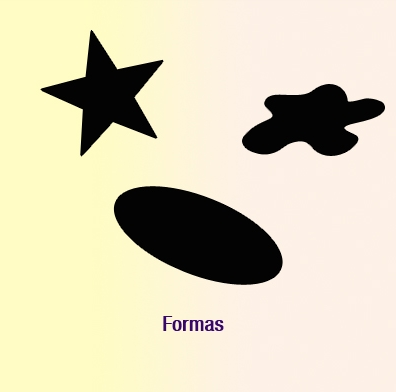
\includegraphics[scale=0.35]{la-forma.png}
    \end{figure}

    La formas pueden encontrarse entre sí de diferentes maneras:

    \begin{enumerate}[label=(\alph*)]
        \item \textbf{Distanciamiento}: ambas formas están separadas entre sí.
        \item \textbf{Toque}: si las acercamos anulamos el espacio entre ellas hasta tocarse.
        \item \textbf{Superposición}: si las acercamos aún mas, una se cruza encima de la otra.
        \item \textbf{Penetración}: igual que \textbf{(c)} pero ambas aparecen transparentes, no hay arriba y abajo y los contornos siguen siendo visibles.
        \item \textbf{Unión}: igual que \textbf{(c)} pero ambas formas quedan reunidas y se convierten en una nueva forma.
        \item \textbf{Sustracción}: cuando una forma negativa se cruza con una forma positiva.
        \item \textbf{Intersección}: igual que \textbf{(d)} pero solamente vemos la porción donde las formas se cruzan.
        \item \textbf{Coincidencia}: si acercamos las formas hasta coincidir, obtenemos una única forma.
    \end{enumerate}

    \begin{figure}[H]
        \centering
        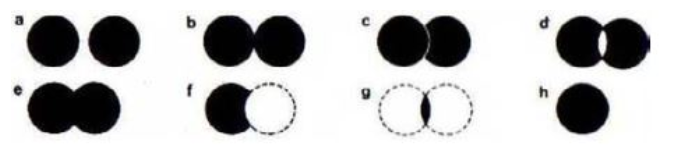
\includegraphics[scale=0.50]{la-forma-encuentro.png}
    \end{figure}

    \item \textbf{Medida}: todas las formas tienen un volumen o una dimensión. El tamaño de las formas se puede establecer de forma relativa, por comparación de unas con otras, pudiendo así decir que una forma es más grande o pequeña que otra, pero en cualquier caso, es físicamente medible.

    \begin{figure}[H]
        \centering
        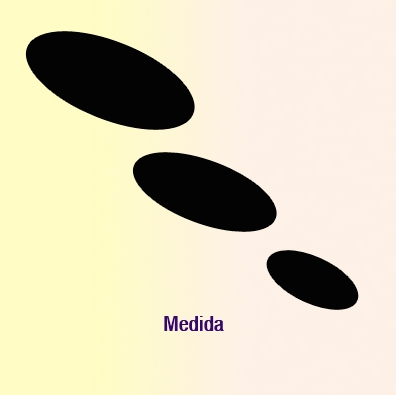
\includegraphics[scale=0.35]{la-medida.png}
    \end{figure}

    \item \textbf{Color}: todo lo que vemos en el mundo tiene color. Las cosas que vemos no solo se diferencia por su forma o tamaño, sino también por su color. El color, y el contraste de color en particular, se usa para llamar la atención sobre una parte determinada de una imagen.

    \begin{figure}[H]
        \centering
        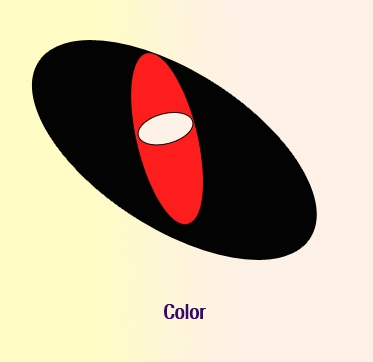
\includegraphics[scale=0.35]{el-color.png}
    \end{figure}

    \item \textbf{Textura}: es la característica visual o táctil de todas las superficies. El material con el que se hacen los objetos le aporta unas determinadas características como rugosidad, suavidad, aspereza, homogeneidad, etc...

    \begin{figure}[H]
        \centering
        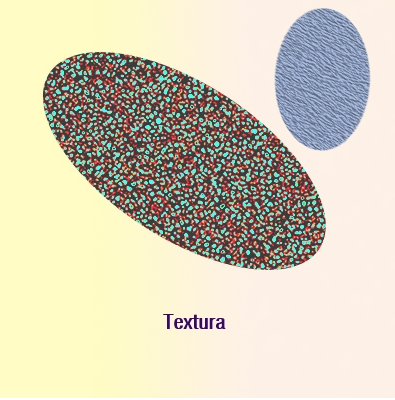
\includegraphics[scale=0.35]{la-textura.png}
    \end{figure}
\end{itemize}

\subsection{Elementos de Relación: Dirección, Posición, Espacio y Gravedad}
Este grupo de elementos gobierna la ubicación y la interrelación de las formas que componen un diseño. Algunos como la posición y la dirección pueden ser percibidos mientras que otros como el espacio o la gravedad se pueden sentir.

\begin{itemize}
    \item \textbf{Dirección}: la dirección de una forma depende de su relación con el observador, el marco que la contiene o con otras formas cercanas con cuales se compara.

    \begin{figure}[H]
        \centering
        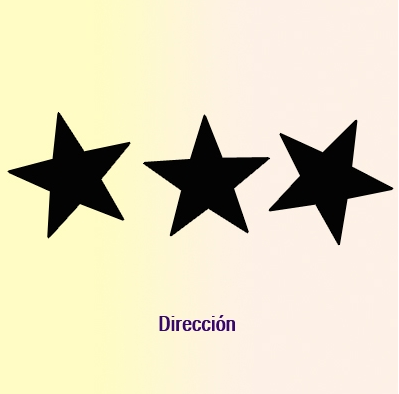
\includegraphics[scale=0.35]{la-direccion.png}
    \end{figure}

    \item \textbf{Posición}: la posición de una forma es juzgada respecto al cuadro que la contiene o la estructura global del diseño.

    \begin{figure}[H]
        \centering
        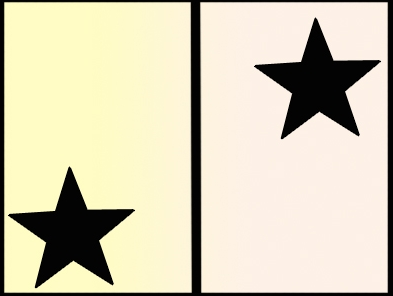
\includegraphics[scale=0.35]{la-posicion.png}
    \end{figure}

    \item \textbf{Espacio}: las formas, por muy pequeñas que sean, siempre ocupan un espacio. Así, el espacio puede estar ocupado o vacío. Se puede usar la perspectiva para simular o sugerir la ilusión de profundidad. Se pueden superponer objetos de forma que el observador perciba como más cercano el que esta delante de los demás. También podemos lograr la profundidad en el campo visual con la utilización de contraste y la variación de tamaño de las formas.

    \begin{figure}[H]
        \centering
        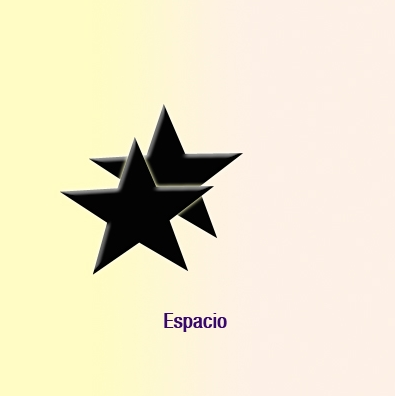
\includegraphics[scale=0.40]{el-espacio.png}
    \end{figure}

    \item \textbf{Gravedad}: la sensación de gravedad no es visual, sino psicológica. Tendemos a aplicar cualidades tales como pesadez o ligereza, estabilidad o inestabilidad, tanto a las formas individuales como a los grupos de formas.

    \begin{figure}[H]
        \centering
        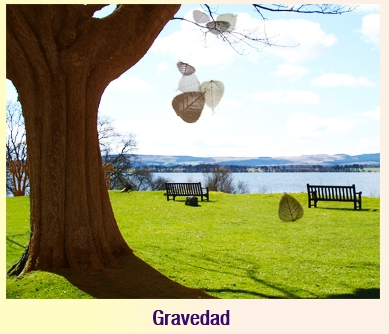
\includegraphics[scale=0.35]{la-gravedad.png}
    \end{figure}
\end{itemize}

\subsection{Elementos Prácticos: Representación, Significado y Función}
Los elementos prácticos del diseño permanecen ocultos en el contenido y la trascendencia del diseño. Estos elementos son:

\begin{itemize}
    \item \textbf{Representación}: una forma es representativa cuando se deriva del mundo natural o del mundo hecho por el ser humano. la representación puede ser \textbf{realista}, \textbf{estilizada} o \textbf{medio abstracta}. Una fotografía de un documento es una representación realista del mismo. Un dibujo de los perfiles de dicho documento es una representación estilizada. Un dibujo naif de dicho documento es una representación medio abstracta.

    \begin{figure}[H]
        \centering
        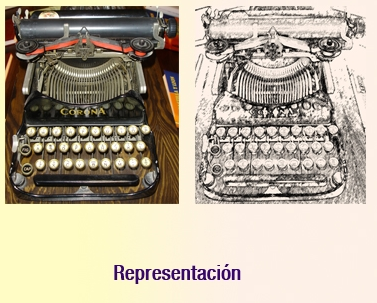
\includegraphics[scale=0.45]{la-representacion.png}
    \end{figure}

    \item \textbf{Significado}: es la imagen conceptual que se representa en nuestra mente cuando el diseño transporta un mensaje visual. Cada receptor del mensaje dará una interpretación y un significado distinto, según sean sus conocimientos y experiencias.

    \begin{figure}[H]
        \centering
        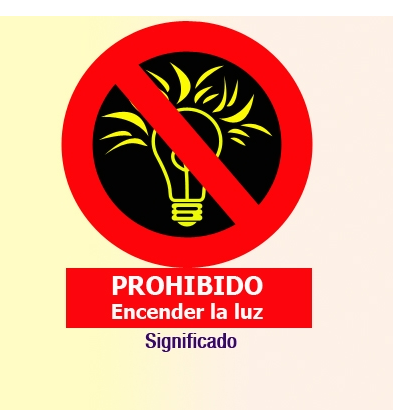
\includegraphics[scale=0.40]{el-significado.png}
    \end{figure}

    \item \textbf{Función}: la función se hace presente cuando un diseño debe servir a un determinado propósito. La imagen anterior, por ejemplo, cumple una función muy importante. Colocada en el lugar adecuado, como una sala de revelado, cumple la función de mantener el ambiente oscuro para poder trabajar.
\end{itemize}

\section{Interfaces Web}
El número de usuario de internet aumenta día a día, y el número de páginas Web también. Internet a cambiado, no solo la forma de trabajar sino también la forma en la que nos relacionamos.

Creamos páginas web para poder comunicar cosas a través de internet. Creamos páginas de tipo personal donde publicamos nuestras opiniones, nuestras fotos, nuestros viajes, etc. También creamos páginas con las que pretendemos obtener algún beneficio económico.

Todas y cada una de estas páginas son creadas con alguna finalidad. Lograr nuestro objetivo dependerá en gran medida de la eficacia del diseño que realicemos.

En \href{https://es.wikipedia.org/wiki/World_Wide_Web}{esta entrada de Wikipedia} tiene información importante que debes conocer sobre la \textbf{World Wide Web}, como su historia, estándares y tecnologías. Debes consultar también los enlaces de cada uno de los estándares.

\subsection{Interacción Persona-Ordenador}

La \textbf{IPO} (Interacción Persona-Ordenador) es la disciplina que estudia el intercambio de información entre personas y ordenadores. Cuando hay una buena interacción entre el usuario y ordenador el intercambio de información es más eficiente, hay menos errores y la satisfacción de la persona es mayor.

Hoy en día la mayor parte de los sistemas informáticos son interactivos y su éxito radica en gran medida en la eficacia del diseño de la interfaz persona-ordenador. Por ello, la interfaz debe estar diseñada pensando en las necesidades del usuario.

Debemos tener en cuenta que cada día es mayor el número de personas que utiliza el ordenador, y que estas personas se enfrentan a este tipo de interacción con diferentes niveles de formación y perspectiva.

\subsection{Diseño de una Interfaz Web: Objetivos}
Una \textbf{interfaz Web} es un \textbf{sistema gráfico} que permite a los usuarios acceder a los contenidos de la Web mediante diferentes elementos gráficos, los cuales son conocidos por la gran mayoría de usuarios que accederán a nuestra web.

El \textbf{objetivo principal} en el diseño de una interfaz Web es que sus usuarios puedan acceder a todos los contenidos de la forma más rápida y simple posible.

Para que el \textbf{diseño web} sea \textbf{efectivo}, debemos diseñar una interfaz que cobra todos nuestros objetivos. Este diseño debe facilitar que nuestros usuario puedan acceder con facilidad a todo el contenido, puedan interactuar con eficacia con todos sus componente y de forma satisfactoria.

Para conseguir dicho objetivo debemos tener en cuenta las siguiente pautas:

\begin{itemize}
    \item La paciencia de las personas no es ilimitada. Si una persona entra en una web y no encuentra rápidamente la información que esta buscando no permanecerá mucho tiempo.
    \item El gusto, considerado como una cuestión de preferencias estéticas, varia mucho de una persona a otra, pero no debemos olvidar que un diseño cuidadoso, una interfaz agradable y un uso coherente de los elementos gráficos nunca nos hará perder usuarios.
    \item Los enlaces que no funcionan o que no redirigen a la información que prometían generan en el visitante una sensación de rechazo, con la consiguiente perdida de confianza en nuestra página, llegando incluso a la determinación de no volver a visitarla de nuevo.
\end{itemize}

A la hora de \textbf{realizar el diseño} de una página web existen \textbf{diferentes filosofías} o \textbf{estrategias}. Nosotros vamos a comentar las dos más empleadas actualmente:

\begin{itemize}
    \item \textbf{Diseño Responsivo o Adaptativo}: hoy en día cuando diseñamos una aplicación debemos pensar que ésta no se va solo a visualizar en un mismo tipo de dispositivo, así que cuando la estamos diseñando tenemos que tener en cuenta los diferentes tipos de dispositivos en los que se va a visualizar. Habitualmente se desarrolla la página web primero para un ordenador y posteriormente tenemos que indicar como se va a visualizar esta en otros dispositivos como tablets, móviles, etc. Dichos cambios pueden consistir en modificar o cambiar el aspecto, o incluso en eliminar algunos elementos del diseño.

    \item \textbf{Diseño Mobile First}: actualmente esta cambiando la tendencia sobre visualización de contenido web, y mientras durante mucho tiempo las webs se han visualizado el ordenador como dispositivo principal, actualmente son los dispositivos móviles donde más páginas web se ven. Teniendo en cuenta esto, lo que persigue esta filosofía es realizar el diseño primero para un dispositivo móvil y posteriormente realizar las modificaciones oportunas para que se adapte a otro tipo de dispositivos como ordenadores.
\end{itemize}
% Bibliography

\addcontentsline{toc}{chapter}{Bibliografía}
\bibliography{citas}
\bibliographystyle{unsrt}

\end{document}